\section{Neural Networks}
\subsection{Perceptron:} A perceptron is a single layer neural network that can be used for classification. The perceptron is a linear classifier that uses the \emph{Heaviside step function} as its activation function. The perceptron is trained using the \emph{perceptron learning algorithm} which is a type of \emph{supervised learning}. The perceptron learning algorithm attempts to learn a weights \(\mathbf{W}\) matrix and bias vector \(\mathbf{b}\) that can be used to classify new inputs according to the formula:
\[\hat{y}=\begin{cases}
    1 & \text{if } \mathbf{W}^T\mathbf{x}+\mathbf{b}\geq0\\
    0 & \text{otherwise}
\end{cases}\]
The \textbf{Perceptron Algorithm:}
\begin{enumerate}
    \item Initialize the weights \(\mathbf{W}\) to small random values.
    \item For each training example \((\mathbf{x},y)\) do the following:
    \begin{enumerate}
        \item Predict \(\hat{y}\) using the current weights \(\mathbf{W}\).
        \item Update \(\mathbf{W}^{(t+1)}=\mathbf{W}^{(t)}+\eta(y-\hat{y})\mathbf{x}\)
    \end{enumerate}
    \item Repeat step 2 until convergence.
\end{enumerate}
\subsection{Feedforward Multilayer Perceptron:} A feedforward multilayer neural network is a neural network that consists of an input layer, one or more hidden layers, and an output layer. Below is a diagram of a feedforward multilayer neural network with two hidden layers, each consisting of 5 neurons and an output layer consisting of 2 neurons. This network accepts 4 input features and produces 2 output features. The bias term is omitted for simplicity.
%tikz graph of neural network with one hidden layer
\begin{center}
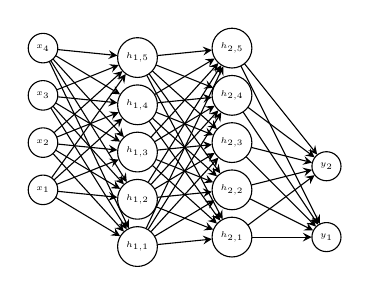
\begin{tikzpicture}[scale=0.6,transform shape,>=stealth,font=\tiny]

% draw input layer
\foreach \i in {1,...,4}
{
  \node[circle,draw=black,minimum size=6mm] (inp\i) at (0,\i) {$x_\i$};
}

% draw hidden layers
\foreach \h in {1,...,5}
{
  \node[circle,draw=black,minimum size=6mm] (hid1\h) at (2,\h-1.2) {$h_{1,\h}$};
  \node[circle,draw=black,minimum size=6mm] (hid2\h) at (4,\h-1) {$h_{2,\h}$};
}

% draw output layer
\foreach \o in {1,2}
{
  \node[circle,draw=black,minimum size=6mm] (out\o) at (6,1.5*\o-1.5) {$y_\o$};
}

% connect input layer to first hidden layer
\foreach \i in {1,...,4}
{
  \foreach \h in {1,...,5}
  {
    \draw[->] (inp\i) -- (hid1\h);
  }
}

% connect first hidden layer to second hidden layer
\foreach \h in {1,...,5}
{
  \foreach \hh in {1,...,5}
  {
    \draw[->] (hid1\h) -- (hid2\hh);
  }
}

% connect second hidden layer to output layer
\foreach \h in {1,...,5}
{
  \foreach \o in {1,2}
  {
    \draw[->] (hid2\h) -- (out\o);
  }
}

\end{tikzpicture}
\end{center}

\subsubsection{Activation Functions:} Activation functions are used to introduce non-linearity into the neural network. The activation function is applied to the weighted sum of the inputs to a neuron. The activation function is typically a non-linear function such as the sigmoid function, the hyperbolic tangent function, or the rectified linear unit (ReLU) function. The sigmoid function is defined as \(\sigma(x)=\frac{1}{1+e^{-x}}\). The hyperbolic tangent function is defined as \(\tanh(x)=\frac{e^x-e^{-x}}{e^x+e^{-x}}\). The ReLU function is defined as \(\text{ReLU}(x)=\max(0,x)\). The ReLU function is typically used in hidden layers and the sigmoid function is typically used in the output layer for binary classification problems. The hyperbolic tangent function is typically used in the output layer for multi-class classification problems.
\subsubsection{Loss Functions:} Loss functions are used to measure the error of the neural network. The loss function is typically a function such as the mean squared error (MSE) function or the cross-entropy function. The cross-entropy function is defined as \(\text{Cross-Entropy}=-\sum_{i=1}^{n}y_i\log{\hat{y}_i}\). The cross-entropy function is typically used in the output layer for classification problems. The MSE function is typically used in the output layer for regression problems. The \emph{MSE function} is defined as \[\text{MSE}=\frac{1}{n}\sum_{i=1}^{n}(y_i-\hat{y}_i)^2\]
\subsubsection{Backpropagation:} At each iteration of training, data is fed through the network until it reaches the output layer. The error is then calculated using the loss function. The error is then propagated backwards through the network using the chain rule to calculate the gradient of the loss function with respect to the weights and biases. The weights and biases are then updated using gradient descent. The process is repeated until convergence. The update equations for gradient descent are as follows:\\
\textbf{Weights:} \[\mathbf{W}^{(t+1)}=\mathbf{W}^{(t)}-\eta\frac{\partial\mathcal{L}}{\partial\mathbf{W}}\] 
\textbf{Biases:} \[\mathbf{b}^{(t+1)}=\mathbf{b}^{(t)}-\eta\frac{\partial\mathcal{L}}{\partial\mathbf{b}}\]
\subsection{Hamming Networks}
Hamming Networks use a feedforward multilayer perceptron architecture followed by a recurrent layer. The recurrent learns prototypes patterns / feature vectors typically present in members of each class. The neuron associated with that prototype indicated the pattern closest to the input.
\subsubsection{The Feedforward Layer:}
The feedforward layer has linear activation function \(\mathbf{f}_{{\scaleto{(1)}{6pt}}}\) is given by: 
\[\mathbf{a}{\scaleto{(1)}{6pt}}=\mathbf{f}_{\scaleto{(1)}{6pt}}\left(\mathbf{W}^T_{\scaleto{(1)}{6pt}}\mathbf{x}+\mathbf{b}_{\scaleto{(1)}{6pt}}\right)\]
The feedforward layer measures the correlation of the input with the prototype each of the prototypes. Input-protype similarity is determined using the matrix \(\mathbf{W}_{\scaleto{(1)}{6pt}}\) where the columns of the matrix are set to be the prototype patterns. Let the prototype patterns be \(\mathbf{p}_1,\mathbf{p}_2,\dots,\mathbf{p}_n\) where \(\mathbf{p}_i\) is the prototype pattern for class \(i\). The matrix \(\mathbf{W}_{\scaleto{(1)}{6pt}}\) and bias vector \(\mathbf{b}_{\scaleto{(1)}{6pt}}\) are defined as:
\[
\mathbf{W}_{\scaleto{(1)}{6pt}}=
    \begin{bmatrix}
        \mathbf{q}_1 & \mathbf{q}_2 & \cdots & \mathbf{q}_K
    \end{bmatrix},\  
        \mathbf{b}_{\scaleto{(1)}{6pt}}=\begin{bmatrix}
            p & p & \cdots & p
    \end{bmatrix}_{K\times 1}^T
\]%
where \(K\) is the number of prototype patterns/classes and is equal to the number of neurons in the first layer \(S_{\scaleto{(1)}{6pt}}\). This choice of \(\mathbf{W}_{\scaleto{(1)}{6pt}}\) and \(\mathbf{b}_{\scaleto{(1)}{6pt}}\) ensures that the output of the first layer is the correlation of the input with each of the prototype patterns because the inner product measures the angles between the prototype vector and the new input, the \(p\) term ensures that the output is positive, and the ReLU function ensures that the output is non-negative. The output of the first layer is then fed into the recurrent layer.\\
\subsubsection{The Recurrent Layer:} The recurrent layer is initialized by the output of the first layer like \( \mathbf{a}_{\scaleto{(1)}{6pt}}(0)= \mathbf{a}_{\scaleto{(1)}{6pt}}\) and then updated according to:
% \begin{minipage}[b]{0.4\linewidth}
    \begin{equation*}
        \mathbf{a}_{\scaleto{(0)}{6pt}}\gets \mathbf{W}^T_{\scaleto{(1)}{6pt}}\mathbf{x}+\mathbf{b}_{\scaleto{(1)}{6pt}},\quad\text{ and }\quad
%     \end{equation*}
% % \end{minipage}%
% % {\hfill\color{gray}\vrule\hfill}%
% % \begin{minipage}[b]{0.5\linewidth}
%     \begin{equation*}
        \mathbf{a}_{\scaleto{(2)}{6pt}}(t+1)=\mathbf{f}_{\scaleto{(2)}{6pt}}
    \left(
        \mathbf{W}^T_{\scaleto{(2)}{6pt}}\mathbf{a}_{\scaleto{(2)}{6pt}}(t)
    \right)
    \end{equation*}
% \end{minipage}%
where \(\mathbf{f}_{\scaleto{(2)}{6pt}}=\max(0,x)\) is the ReLU activation function of the recurrent layer. 

The weight matrix \(\mathbf{W}_{\scaleto{(2)}{6pt}}\) for the recurrent layer is initialized with:
\[
    \mathbf{W}_{\scaleto{(2)}{6pt}}=
        \begin{bmatrix}
            1 &&  -{\scaleto{\epsilon}{9pt}}\\
            &\ddots&\\
            -{\scaleto{\epsilon}{9pt}}&&1
        \end{bmatrix}_{K\times K}
\]
where \(\epsilon < \frac{1}{S-1}\). The feedforward layer acts like an indicator where the most strongly correlated protype transmits the largest signal to the recurrent layer. The recurrent layer then iteratives reapplies the weight matrix until features with lower correlation eventually drop out. Upon convergence, a prediction is made.\\
\begin{center}
\noindent\color{mypink}\rule{4cm}{0.4pt}\\
\emph{\textbf{Neurons that fire together, wire together.}} \\
\(\quad \quad \quad \quad \quad \quad \quad \quad\quad \quad\) - Donald Hebb\\
\noindent\color{mypink}\rule{3cm}{0.4pt}\\
\end{center}
\subsection{Hopfield Networks}
Hopfield networks are a type of recurrent neural network that can be used for classification and optimization. Hopfield networks are composed of a set of neurons that are connected to every other neuron. 
\subsubsection{Recurrent Layer Structure}
The recurrent layer is initialized with the input \(\mathbf{x}\). The structure of the recurrent layer is as follows:
\[\mathbf{a}(0)\gets\mathbf{x},\quad\text{ and }\quad\mathbf{a}(t+1)=\mathbf{f}\left(\mathbf{W}^T\mathbf{a}(t)\right)\]
where \(\mathbf{f}\) is the activation function of the recurrent layer. The activation function of the recurrent layer is typically the sign function, hyperbolic tangent function, or the \emph{saturated linear function (SLF)} which is defined as:
\[\texttt{SLF}(n)=\begin{cases}
    1 & \text{if } n\geq 1\\
    n & \text{if } 0\leq n\leq 1\\
    0 & \text{otherwise}
\end{cases}\]
The weight matrix \(\mathbf{W}\) is initialized with \(K\) prototype patterns \(\mathbf{q}_1,\mathbf{q}_2,\dots,\mathbf{q}_K\) where \(\mathbf{q}_k\) is the prototype pattern for class \(k\). The weight matrix \(\mathbf{W}\) is defined as:
\[\mathbf{W}=\sum_{k=1}^K\mathbf{q}_k{\mathbf{q}}_k^T\]
where \(k\) is the class of the prototype pattern and \(K\) is the number of neurons in the network. The result is a square weight matrix \(\mathbf{W}\in\mathbb{R}^{K\times K}\). The iterative process for classification in the recurrent network is as follows:
\[\mathbf{a}(0)\gets\mathbf{x}\] 
\[\implies\quad\mathbf{a}(t+1)=\texttt{SLF}\left(\sum_{k=1}^K\mathbf{q}_k({\mathbf{q}_k}^T\mathbf{x})\right)\]
The quantity scalar quantity \(\alpha_k=\mathbf{q}_k^T\mathbf{x}\) is the correlation of the input with the prototype pattern \(\mathbf{q}_k\). The recurrent process is repeated until the output converges. The output of the network is the class of the prototype pattern that the input is most correlated with. 
\subsection{Supervised Hebbian Learning}
Supervised Hebbian learning is a type of supervised learning that is based on the idea that when neurons on both sides of a synapse are activated, the synapse is strengthened. 
\subsubsection{Linear Associator}
A linear associators is an example of a neural network called an associative memory. The goal of the associator is to learn \(K\) prototype input-output vectors that satisfy:
\[\mathbf{a}=\mathbf{W}^T\mathbf{x}\]
The network should recall input-output pairs it has encouneter and also remain \emph{robust} by ensuring that a small amount of noise to the input only results in a small shift in the prediction.
\subsubsection{The Supervised Hebbian Learning Algorithm}
We initialize the weight matrix \(\mathbf{W}=0\) and then update the weight matrix using the following iterative process:
\emph{\textbf{for each training example \((\mathbf{x}_k,\mathbf{y}_k)\) do the following:}}
\[
    \mathbf{W}^{{\scaleto{(\text{new})}{6pt}}}\gets\mathbf{W}^{{\scaleto{(\text{old})}{6pt}}}+\mathbf{x}_k\mathbf{y}_k^T    
\]